\section{Problem 2: Decisions for Drivers and Analysis for the Decision Model}
\subsection{Data Preparing}
\begin{enumerate}
\item \textbf{Raw Data} \\
The overview of taxi data and flight data is shown in the form of data distribution statistics chart as followed.And the detailed datas are placed in appendix.
\begin{figure}[H]
\centering
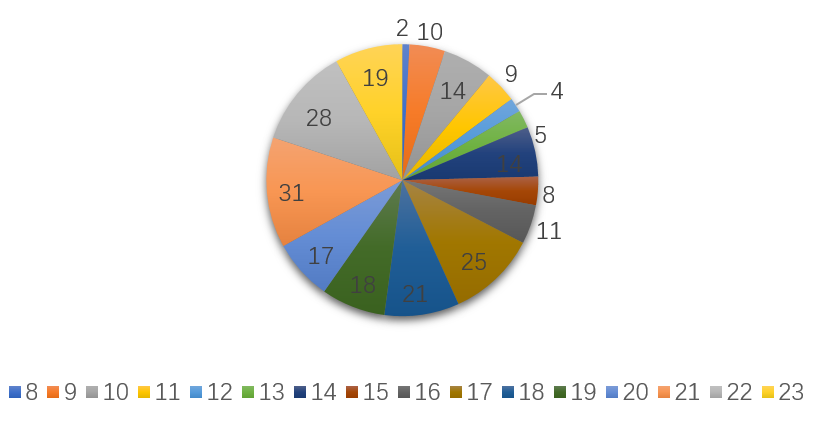
\includegraphics[width=0.7\textwidth]{figures/Q2_1.png}
\caption{Flight data of Pudong Airport 20180602 obtained by crawling}
\label{fig:label}
\end{figure}

\begin{figure}[H]
\centering  
\subfigure[Passenger distance distribution of taxi in Shanghai in 2015]{
\label{Fig.sub.q2111}
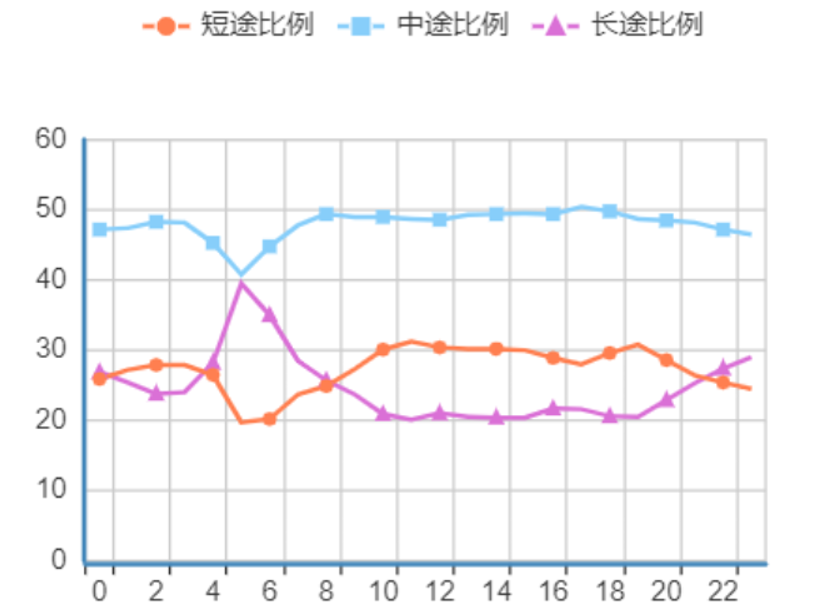
\includegraphics[width=0.45\textwidth,height = 4cm]{figures/Q2_2.png}}
\subfigure[Average speed distribution of taxis in Shanghai in 2015]{
\label{Fig.sub.q2112}
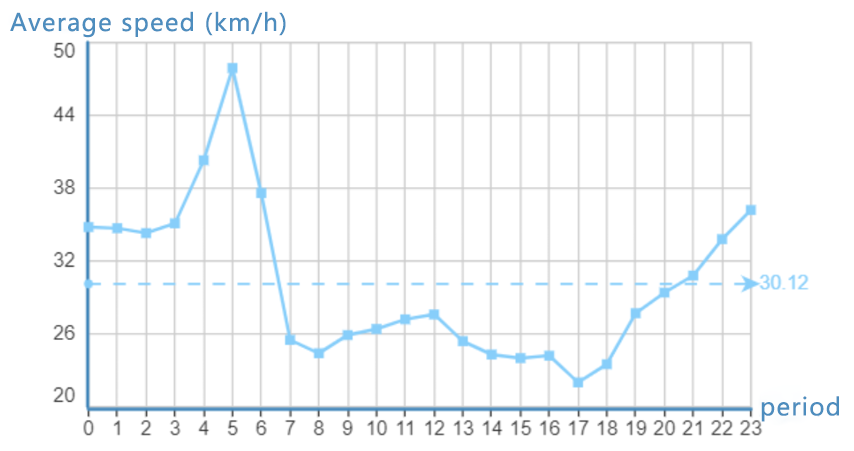
\includegraphics[width=0.45\textwidth,height = 4cm]{figures/Q2_3.png}}
\caption{ Taxi Data }
\label{Fig.q211}
\end{figure}

\item \textbf{Processed Data} \\

\begin{figure}[H]
\centering
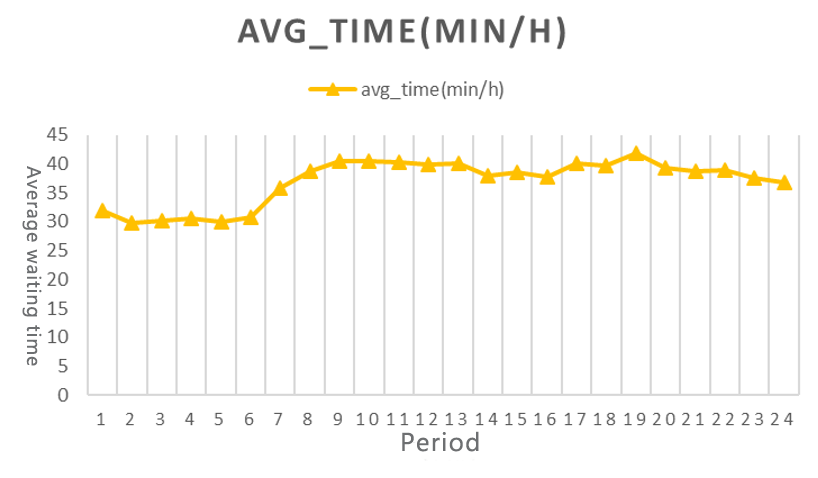
\includegraphics[width=0.7\textwidth]{figures/Q2_4.png}
\caption{Average waiting time of receiving orders in urban areas in different time periods}
\label{fig:label}
\end{figure}
From the raw data, we do a lot of processing, and finally extract 2077 pieces of data as clustering candidate data.And the field is shown in below table.And we put forward some assumptions: If the taxi enters Pudong Airport in empty state at $t_{empty}$ and becomes loaded at $t_{busy}$, the starting time of queuing is assumed to be $t_{empty}$. If the taxi enters the airport in loaded state and becomes empty at $t_{empty}$ and becomes loaded at  $t_{busy}$ again, the starting time of queuing is assumed to be $t_{empty}$.
\begin{table}[H]
\centering
\caption{Candidate data for clustering}
\begin{tabular}{|l|p{5cm}|p{7cm}|}
\hline
\textbf{Field} & \textbf{Description} & \textbf{Calculate Method} \\ \hline
$Id$ & taxi number & from origin data \\ \hline
$Time$ &  the time begin queuing at Pudong Airport & from origin data  \\\hline
$Wait\_time$ & taxi queuing time in airport & $t_{busy} - t_{empty}$  \\ \hline
$taxi\_density$ & Accumulated number of taxis in Pudong airport within 2 hours ahead of $Time$ & Use a set to record all the unique taxi number in these two hours, and the size of the set is the taxi density.\\ \hline
$flight\_density$ & Total number of passengers landing at Pudong airport within 2 hours ahead of $Time$ & Sum of the total number of passengers of the flight with the planned landing time in these two hours\\ \hline
\end{tabular}
\end{table}
\end{enumerate}



\subsection{Parameter Calibration}

\begin{table}[H]
\centering
\caption{ Parameter Setting for Model}
\begin{tabularx}{15cm}{llX}  % 10cm 減去前兩個欄位寬度後,剩下的通通給
\hline                      % 第三欄位使用,文字超出的部份會自動折行
Symbol & Value  & Meaning  \\
\hline
${L}_1$  & 46.4 & Unit: km, the approximate distance from Pudong Airport To Downtown\\
${t}_DE$ & 0.576014 & Unit: H, the average waiting time of passengers in the queue in this period, selected from the clustering result set, time point is 19:17 \\
$\alpha$  & 1 & Weather factor, for the convenience of calculation, it is assumed that the weather is in good condition\\
${V}_2$ & $f(t)$ &Unit: km/h, average speed in urban area,$f(t)$ is the function to calculate ${V}_2$ \\
${V}_1$   & 64.7 & Unit: km/h, average speed from Pudong to downtown\\
$\beta$  & 1 & Road condition factor, also assuming good road condition\\
$o$  & 0.088 & Unit: L/km, fuel consumption per mileage\\
$k$  & 7.13 & Unit: \textyen/L, unit oil price\\
${f}_1$  & 14 & Unit: \textyen, starting price of taxi in Shanghai\\
$a$  & 3 & Unit: km, first gradient mileage limit\\
${f}_2$  & 2.5 & Unit: \textyen, more than 2.5 \textyen/km over $a$\\
$b$  & 15 & Unit: km, first gradient mileage limit\\
${f}_3$  & 3.6 & Unit: \textyen, over part B, 3.6 \textyen/km\\
$\mu$  & 0.15 & Weighting factors for time periods\\
\hline
\end{tabularx}
\label{parameter_setting}
\end{table}


\subsection{Model Calculation}

After standardizing the candidate data, 1000 pieces of 2077 pieces of data are randomly selected as samples. Each sample is $(time, flight\_density, taxi\_density, wait\_time)$, which corresponds to the parameter $(T,{N}_a,{N}_c,{t}_q)$ in Task 1, we set $k = 4,5,6,7$ for K prototype clustering, and bring $k$  into the following formula:
\[E = \sum_{i=1}^{k} \sum_{i=1}^{n} {D}_s({X}_i,{X}_{center})\]
Calculating the mean square error of each cluster set under each $k$ value:
\begin{table}[H]
\caption{Mean Square Deviation}
\begin{center}
\begin{tabularx}{5cm}{p{2cm}|p{3cm}}
\hline
K & E  \\
\hline
4 & 100.56  \\
5 & 35.94 \\
6 & 165.67  \\
7 & 189.86 \\
\hline
\end{tabularx}
\end{center}
\end{table}
It can be concluded from above table that the clustering effect is  best when $k = 5$, and the clustering diagram after clustering is as follows:
\begin{figure}[H]
\centering
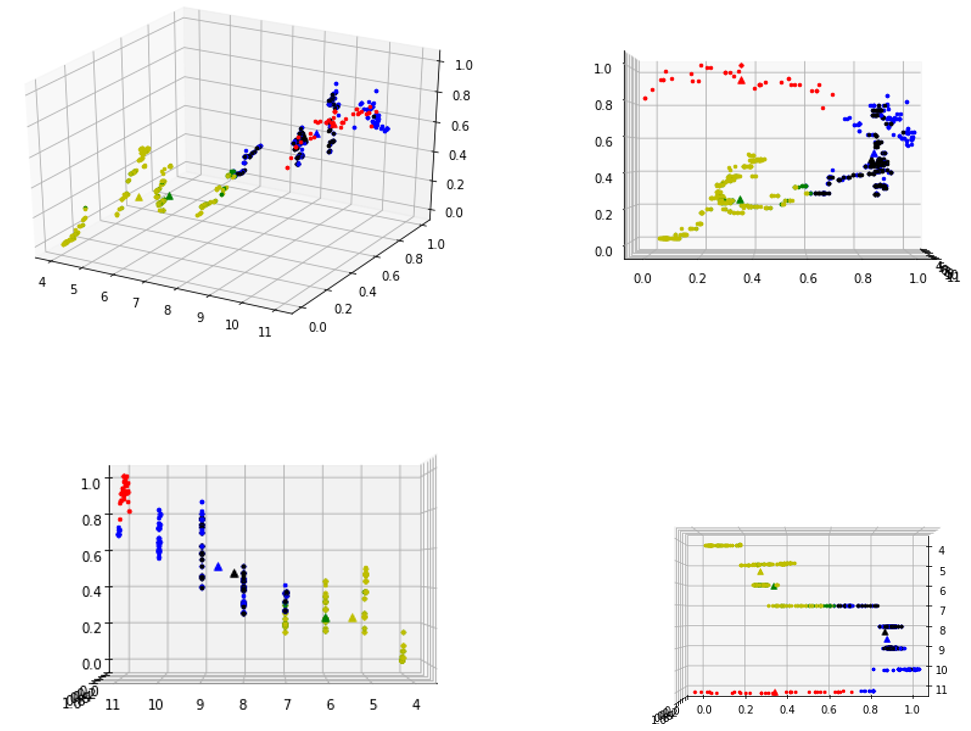
\includegraphics[width=0.7\textwidth]{figures/Q2_5.png}
\caption{Distribution of Clustering Results}
\label{fig:label}
\end{figure}
When $k = 5$, cluster sets and cluster centers are saved for the following calculation. Then, 50 pieces of data are randomly selected from 2077 pieces of data as decision samples (excluding the $wait\_time$ field, and the data is in the appendix), and brought into model. The net profit of each sample in the queue and the net profit returned to the urban area are calculated. The overall comparison chart is as follows:

\begin{figure}[H]
\centering  
\subfigure[Net income per unit time - Number of passengers]{
\label{Fig.sub.q2111}
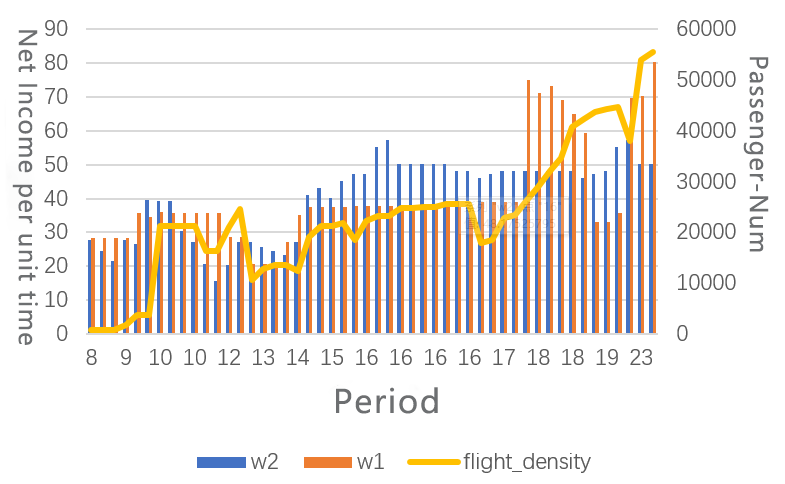
\includegraphics[width=0.45\textwidth,height = 5cm]{figures/Q2_6.png}}
\subfigure[Net income per unit time -Number of taxis]{
\label{Fig.sub.q2112}
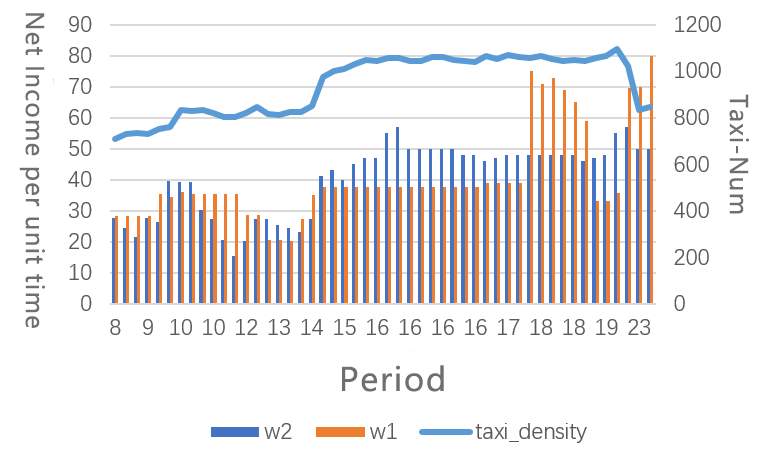
\includegraphics[width=0.45\textwidth,height = 5cm]{figures/Q2_7.png}}
\caption{Comparison of overall results}
\label{Fig.q211}
\end{figure}
According to the above figures, we can see the decision scheme made by the model:
\begin{table}[H]
\centering
\caption{ Decision Plan}
\begin{tabularx}{15cm}{lX}  
\hline                      
Decision & Period   \\
\hline
Queue up  & $8:00-9:00 \;\&\; 11:00-12:30 \;\&\; 18:00-19:00 \;\&\; 22:00-24:00$\\
Return to urban & $9:00-11:00 \;\&\; 12:30-18:00 \;\&\; 19:00-22:00$\\
\hline
\end{tabularx}
\end{table}
This plan is the choice we give to taxi drivers in this airport.

\subsection{Rationality Analysis}
The decision calculated by our model has the following characteristics:

\begin{enumerate}
\item Tend to choose a later night (such as 22:00-24:00), which is consistent with the actual situation of life. Because the choice of public transport at night becomes scarce, the probability of flight passengers choosing to take taxis will increase. Just as the proportion of night flight passengers choosing taxis in Pudong Airport calculated by China Daily is as high as 45\%, in this case, the demand for taxis will be large, and the waiting time of drivers will be shortened. In addition, the charge of night taxi is higher, especially in the airport where the order receiving rate is probably long-distance, the driver's income will increase significantly. Therefore, drivers will naturally prefer to wait in line for passengers in this period of time.
\item Tend to make the choice of waiting in line at the peak of urban traffic (18:00-19:00 \& 8:00-9:00). In fact, it is also easy to understand that when the urban area is in the rush hour of going to and from work, the road is blocked and the average traffic jam time is long, which will lead to the decrease of the driver pick-up frequency, the increase of the air run time and the increase of the fuel consumption, so the taxi drivers are more inclined to avoid such peak periods.
\item Tend to make the choice of waiting in line when the passenger demand is small (11:00-12:30). In the period of noon, according to people's normal life, they are at the time of lunch. At this time, the demand for taxis in the urban area is bound to be small.
\item  In other time periods (mostly during the day), the proportion of airport passengers who choose to take taxis is small (only 15\% of Pudong Airport passengers choose to take taxis during the day according to China Daily net). If they queue up, they will waste a lot of time. On the contrary, in the urban area, the road traffic condition is normal, which is more conducive to business.
\end{enumerate}
And about rationality analysis
\begin{enumerate}
\item The parameters such as taxi time interval, average speed distribution, average waiting time for single receipt and taxi pricing are all open real data. At the same time, the extracted airport taxi sample data is obtained through a large number of screening statistics, which is consistent with the actual situation.
\item The clustering model used to calculate the waiting time of the queue has a better clustering effect. After the evaluation of the silhouette coefficient combining the two factors of cohesion and separation, that is, for each vector in K clusters, the silhouette coefficient\cite{kaufman2009finding} of each vector is calculated by the following formula:
\begin{equation} S(i) = \frac{b(i)-a(i)}{max(a(i),b(i))}\end{equation}
\end{enumerate}

\subsection{Dependency Analysis}
Our decision model consists of six variables: $N_a$,$N_c$,$L_2$,$V_2$,$t_w$,$T$,and we calculate the average and the maximum, minimum values of them respectively so as to conduct sensitivity analysis. And the values are shown in below table.
\begin{table}[H]
\centering
\caption{Parameter sensitivity analysis}
\begin{tabularx}{15cm}{c|c|c|c|c} 
\hline                    
Parameter & Max & Min & Avg & Description\\
\hline
$N_a$  & 55923 & 740 & 23187 & flight density\\
$N_c$  & 1107 & 703 & 943 & taxi density \\
$L_2$  & 15.5647 & 12.0199 & 12.9387 & taxi carrying distance per order\\
$V_2$  & 47.9 & 22.0 & 30.1375 & taxi average speed in various time\\
$t_w$  & 0.982 & 0.4974 & 0.6155 & average waiting time for receiving orders \\
$T$  & 23 & 8 & 11 & time(in 24 hours)\\
\hline
\end{tabularx}
\end{table}

Set the i parameter $C_i$ of every parameter in $(N_a.N_c,L_2,V_2,t_w)$from its minimum value to the max value with stride $s$:
\begin{equation} s = \frac{C_{i\_max}-C_{i\_min}}{10}\end{equation}
That is $\{C_{i\_min},C\_{i_min}+s,C_{i\_min}+2s,\cdots,C_{i\_max}\}$,and the remaining five parameters are set to average value.Then bring these variables into the decision model, so that we can get $\{d_{w\_i\_1},d_{w\_i\_2},\cdots,d_{w\_i\_10}\}$ where ${d_{w\_i\_k} = w_{1\_i\_k} - w_{2\_i\_k}}$.,So that the ratio of the increment of each $d\_w$ relative to the former to the increment of $C\_i$ can be obtained, that is:
\begin{equation} r_{w\_i\_k+1} = \frac{|\frac{d_{w\_i\_k+1} -d_{w\_i\_k} }{d_{w\_i\_k}}|}{\frac{s}{C_{i\_min}+ks}}\end{equation}
we can get $r_{w\_i} = [0,r_{w\_i\_2},r_{w\_i_3},r_{w\_i\_4},r_{w\_i\_5}]$.By calculating each of the six parameters, a sensitivity matrix of the six parameters can be obtained:
\begin{equation}
r_{w} = 
\left[
\begin{matrix}
 r_{w\_1\_1}  & \cdots & r_{w\_1\_10}      \\
 \vdots  & \ddots & \vdots \\
  r_{w\_6\_1}     & \cdots & r_{w\_6\_10}      \\
\end{matrix}
\right]
\end{equation}
Finally, the average value of each line is obtained:
\begin{equation}
r_{w\_mean} = 
\left[
\begin{matrix}
 r_{w\_1\_mean}       \\
 \vdots \\
  r_{w\_6\_mean}      \\
\end{matrix}
\right]
\end{equation}  
Bring the value of the previous table into the calculation to get $r_{w\_mean}$

\begin{table}[H]
\centering
\caption{ Sensitivity mean value}
\begin{tabularx}{9cm}{lllllll}
\hline                    
 Variable &  $N_a$ & $N_c$ & $L_2$ & $V_2$ & $t_w$ & $T$ \\
\hline
value & 25.26  & 14.37 & 1.59 & 6.78 & -9.43 & 7.12\\
\hline
\end{tabularx}
\end{table}
It can be seen from the above table that: the sensitivity of $N_a$ is the highest, and the sensitivity of $N_c$is the second, that is to say, the decision model has the greatest dependence on flight density $N_a$, and the second is the dependence on taxi density $N_c$.